% Mo Jabeen Template for docs 

\documentclass[11pt]{scrartcl} % Font size

%%%%%%%%%%%%%%%%%%%%%%%%%%%%%%%%%%%%%%%%%
% Wenneker Assignment
% Structure Specification File
% Version 2.0 (12/1/2019)
%
% This template originates from:
% http://www.LaTeXTemplates.com
%
% Authors:
% Vel (vel@LaTeXTemplates.com)
% Frits Wenneker
%
% License:
% CC BY-NC-SA 3.0 (http://creativecommons.org/licenses/by-nc-sa/3.0/)
% 
%%%%%%%%%%%%%%%%%%%%%%%%%%%%%%%%%%%%%%%%%

%----------------------------------------------------------------------------------------
%	PACKAGES AND OTHER DOCUMENT CONFIGURATIONS
%----------------------------------------------------------------------------------------

\usepackage{amsmath, amsfonts, amsthm} % Math packages

\usepackage{listings} % Code listings, with syntax highlighting

\usepackage[english]{babel} % English language hyphenation

\usepackage{graphicx} % Required for inserting images
\graphicspath{{Figures/}{./}} % Specifies where to look for included images (trailing slash required)

\usepackage{booktabs} % Required for better horizontal rules in tables

\numberwithin{equation}{section} % Number equations within sections (i.e. 1.1, 1.2, 2.1, 2.2 instead of 1, 2, 3, 4)
\numberwithin{figure}{section} % Number figures within sections (i.e. 1.1, 1.2, 2.1, 2.2 instead of 1, 2, 3, 4)
\numberwithin{table}{section} % Number tables within sections (i.e. 1.1, 1.2, 2.1, 2.2 instead of 1, 2, 3, 4)

\setlength\parindent{0pt} % Removes all indentation from paragraphs

\usepackage{enumitem} % Required for list customisation
\setlist{noitemsep} % No spacing between list items

%----------------------------------------------------------------------------------------
%	DOCUMENT MARGINS
%----------------------------------------------------------------------------------------

\usepackage{geometry} % Required for adjusting page dimensions and margins

\geometry{
	paper=a4paper, % Paper size, change to letterpaper for US letter size
	top=2.5cm, % Top margin
	bottom=3cm, % Bottom margin
	left=3cm, % Left margin
	right=3cm, % Right margin
	headheight=0.75cm, % Header height
	footskip=1.5cm, % Space from the bottom margin to the baseline of the footer
	headsep=0.75cm, % Space from the top margin to the baseline of the header
	%showframe, % Uncomment to show how the type block is set on the page
}

%----------------------------------------------------------------------------------------
%	FONTS
%----------------------------------------------------------------------------------------

\usepackage[utf8]{inputenc} % Required for inputting international characters
\usepackage[T1]{fontenc} % Use 8-bit encoding

\usepackage{fourier} % Use the Adobe Utopia font for the document

%----------------------------------------------------------------------------------------
%	SECTION TITLES
%----------------------------------------------------------------------------------------

\usepackage{sectsty} % Allows customising section commands

\sectionfont{\vspace{6pt}\centering\normalfont\upshape} % \section{} styling
\subsectionfont{\normalfont\bfseries} % \subsection{} styling
\subsubsectionfont{\normalfont\itshape} % \subsubsection{} styling
\paragraphfont{\normalfont\scshape} % \paragraph{} styling

%----------------------------------------------------------------------------------------
%	HEADERS AND FOOTERS
%----------------------------------------------------------------------------------------

\usepackage{scrlayer-scrpage} % Required for customising headers and footers

\ohead*{} % Right header
\ihead*{} % Left header
\chead*{} % Centre header

\ofoot*{} % Right footer
\ifoot*{} % Left footer
\cfoot*{\pagemark} % Centre footer

\usepackage{array}
\newcolumntype{P}[1]{>{\centering\arraybackslash}p{#1}}
 % Include the file specifying the document structure and custom commands

%----------------------------------------------------------------------------------------
%	TITLE SECTION
%----------------------------------------------------------------------------------------

\title{	
	\normalfont\normalsize
	\vspace{20pt} % Whitespace
	{\huge Intro To Statistical Learning: Notes}\\ % The meh
	\vspace{12pt} % Whitespace
	\rule{\linewidth}{2pt}\\ % Thick bottom horizontal rule
}

\author{\small Mo D Jabeen} % Your name

\date{\normalsize\today} % Today's date (\today) or a custom date

\begin{document}

\maketitle % Print the title

\section{General}

Statsictal is learning is based on making predictions or inferences on data inputs. Via approximating f(x),
where y = f(x) + error.

\subsection{What are the types of statistical problems?}

\begin{itemize}
	\item Regression: Determine outcome variable based on predictors, continous problem ie Range of values 
	\item Classification: Discrete choice of answers (normally qualitative)
	\item Clustering: Determine similar groups of data (no natural output variable)
\end{itemize}

\subsection{Notation}

\begin{equation}
	x_{ij}, i:1,2,\cdots n, j:1,2,\cdots p
\end{equation}
\begin{equation}
	x_{i} = (x{i1},x_{i2},x_{i3} \cdots,x_{ip})
\end{equation}

i is the observation and j is the predictor.

\subsection{What is paramtric and non parametric?}

\textbf{Parametric:} Assume form of the desired function and calculate parameters based on the assumption.\\

\textbf{Non Parametric:} Do not make any explicit assumptions, instead fit function best to the data given.\\

Choosing an non parametric avoids the problem of having a function form very differnt to reality however opens up
the possibility of overfitting (following noise too closely) and needs more data for an accurate form.\\

Furthermore, if the main goal is inference, restrictive (parametric) are much easier to interpret.

\subsection{What is unsupervised learning?}

There is no response/outcome variable, ie clustering.\\

\textbf{Semi supervised learning:} some response variables.

\section{Quality of fit}

Measure how well the model fits the the true model.

\subsection{How is Mean Squared Error used?}

Regression compares the predicted outcome to the true value and measures the MSE. However many
statistical methods minimise the \textbf{training} MSE, therefore a test MSE should be used!\\

If there is a small training MSE and a large test MSE this can indicate overfitting.

\subsection{What is Bias Variance Trade off?}

MSE can be deconstructed to give variance of the estimate function, squared bias of the estimate function
and variance of error.

\begin{equation}
	E(y_o - \hat{f}(x_o))^2 = Var(\hat{f}(x_o)) + (Bias(\hat{f}(x_o)))^2 + Var(\epsilon)
\end{equation}

Aim is to minimise variance and bias as error can not be removed.

The rate of change between var and bias determines optimal flexibilty of a model.

\subsubsection{What is variance?}

The change in outcome/model if the data set is changed. Higher flexibilty of model often increases
this.

\subsubsection{What is bias?}

Error from approximations.

\subsection{Error Rate}

Classification accuracy is measured by error rate, the frequency of values that predicted the wrong class. In this
case test error rate is also preffered.

\begin{equation}
	Error\; rate = \frac{1}{n} \sum{I(y_i \neq \hat{y_i})} , I: y_i \neq \hat{y_i} ? 1:0
\end{equation}

\subsection{What is Bayes Classification?}

Choosing the max probablilty an observation is a class will minimise the error rate.

Ie if there are only two classes, choose the class that fits:
\begin{equation}
	P(Y=1|X=x_o) > 0.5
\end{equation}

\subsection{What is Bayes error rate?}

\begin{equation}
	Bayes\; Error\; Rate = 1 - E(maxP(Y=j|X=x_o))
\end{equation}

E is the average for all values of X. ie if the probablilty of a 2 class, setup where one class is 0.7 the error rate
will be 0.3. Not possible to actually use Bayes as the probablilty is unknown, however, this is the gold standard.

\section{Classification}

\subsection{What is K nearest neighbours?}

KNN identifies the K points closest to training point x, shown as \(\eta_o\). The conditional probablilty is then
the fraction of the points in \(\eta_o\) that equal class j.

\begin{equation}
	P(Y=j|X=X_o) = \frac{1}{K}\sum_{i\epsilon \eta_o}{I(y_i=j)}
\end{equation}

Then classify point x as the class with the highest probablilty. K =1 has low bias but high variance.

\subsection{Why logistic regression instead of linear regression?}

To create a regression problem from a classification, you would be forced to create some type of ordering of the qualitative
variables if >2. This ordering may not be true for the data set. However with a binary classification least squares is possible, the
issue is that least squares does not have the required boundaries for a binary decison ie 0-1 so you would create a useless areas.

\subsection{What is logistic regression?}

To bound p(X) between 0 and 1, exponential equation is used:

\begin{equation}
	p(X) = P(Y=1|X)
\end{equation}

\begin{equation}
	p(X) = \frac{e^{\beta_0 + \beta_1X}}{1+e^{\beta_0 + \beta_1X}}
\end{equation}

This will produce an S curve, and if the log is taken shows that 1 unit increase in X gives a change of log odds by 
\( \beta_1\).

\begin{equation}
	log\; odds: ln(\frac{p(X)}{1-p(X)}) = \beta_0 + \beta_1X
\end{equation}

This also shows that if \(\beta_1\) is postive, increasing X will increase p(X), if negative the increasing X will
decrease p(X).

\subsection{How is logistic regression used?}

For binary class scenarios you are trying to maximise the liklehood function to estimate the beta parameters.

Likelhood function:
\begin{equation}
	(\beta_o,\beta_1) = \Pi_{i:Y_i=1}p(x_i) + \Pi_{i:Y_i=0}(1-p(x_i))
\end{equation}

\subsection{What is standard error?}

\begin{equation}
	SE(\alpha^2) = x
	\label{normalSE}
\end{equation}

\ref{normalSE} shows for each sample expect \(\alpha\) to very by x on average.

The below is the standard erorr of the mean ie std/n:

\begin{equation}
	SE(\mu)^2 = \frac{\sigma^2}{n}
\end{equation}

The below is based on how the Betas are calculated (this is for linear regression):

\begin{equation}
	SE(\hat{\beta_0})^2 = \sigma^2(\frac{1}{n} + \frac{\bar{x}^2}{\sum{(x_i-\bar{x})^2}})
\end{equation}

\begin{equation}
	SE(\beta_1)^2 = \frac{\sigma^2}{\sum{(x_i-\bar{x})^2}}
\end{equation}



\subsection{What ways can you validate the parameters?}

Use confidence intervals, z/t tests and hypothesis tests.\\

The null hypothesis is that there is no relationship between predictor and outcome.

\subsection{What are dummy variables?}

If there is qualitative category for the observational data, this can be used a dummy value which is used to represent
the observations. This then requires new parameters to be calculated.\\

I.e. set \(x_i\) as 1 if male, 0 if female. If more than one category use multiple pairs as preidctors, ie 
\(x_{i1} = X==Asian?1:0, x_{i2} = X==Jamican?1:0\).\\

These parameters from this can be validated in the same way.

\subsection{How do you include multiple predictors in logistic regression?}

Match the number of preidctors to the number of parameters:

\begin{equation}
	\ln\frac{p(x)}{1-p(x)} = \beta_o + \beta_1x_{i1} + \beta_2x_{i2} + \cdots \beta_px_{ip}
\end{equation}

Multiple predictors can show how the interweaving between each other and the outcome. Not shown when not included if 
not included in the equation.\\

Multi-class logistic regression exists but is not really used.

\subsection{What is linear discriminant analysis?}

Model X for each class Y as a distribution, then use Bayes therom and compare all dist to choose the max P(Y=k|X=x).
\textbf{Assumes normal distribution for each class.}

\subsubsection{LDA Equation}

\(\Pi_k\) : Probablilty of the randomly chosen observation X being in class K. (Fraction of observations that belong to the kth class)\\

\(f_k(X)\): Density function for X belonging to class K.

\begin{equation}
	P(Y=k|X=x) = \frac{\Pi_kf_k(x)}{\sum^K_{l=1}{\Pi_lf_l(X)}}
\end{equation}

\begin{equation}
	P(Y=k|X=x) = \frac{Overall\; Prob * density\; of \; x \; for \; k}{\sum_{all\; classes}(Overall\; Prob * density\; of \; x \; for \; k)}
\end{equation}

The focus is estimating f(x) to fit Bayes Classifier. A point on the density function should be maximised as shown by:
\textbf{Assuming the var is common for all classes and a normal dist}

\begin{equation}
	\delta_k(x) = x\frac{\mu_k}{\sigma^2} - \frac{\mu_k^2}{2\sigma^2}
\end{equation}

Calcuating the above may not be possible as the population is not available so estimates of mean and std are used:

\begin{equation}
	\hat{\mu_k} = \frac{1}{n_k}\sum_{i:y_i=k}{x_i}
\end{equation}


\begin{equation}
	\hat{\sigma^2}  = \frac{1}{n-K}\sum^K_1\sum_{i:y_i=k}(x_i - \hat{\mu_k})
\end{equation}

This being the average sample var for each class (on the premise they are common).\\

These are then plugged in to give the boundary points as:

\begin{equation}
	\hat{\delta_k(x)} = x\frac{\hat{\mu_k}}{\hat{\sigma^2}} - \frac{\hat{\mu_k}^2}{2\hat{\sigma^2}}
\end{equation}

If possible compare to Bayes error rate to determine classifier peformance.

\subsubsection{What if the number of predictors > 1?}

Multi-variate normal dist is then used. From which a class specific mean vector is used and a common covariance matrix.\\

Each predictor follows a one dimensional normal dist with some correlation between predictors.

\begin{figure}[h] % [h] forces the figure to be output where it is defined in the code (it suppresses floating)
	\centering
	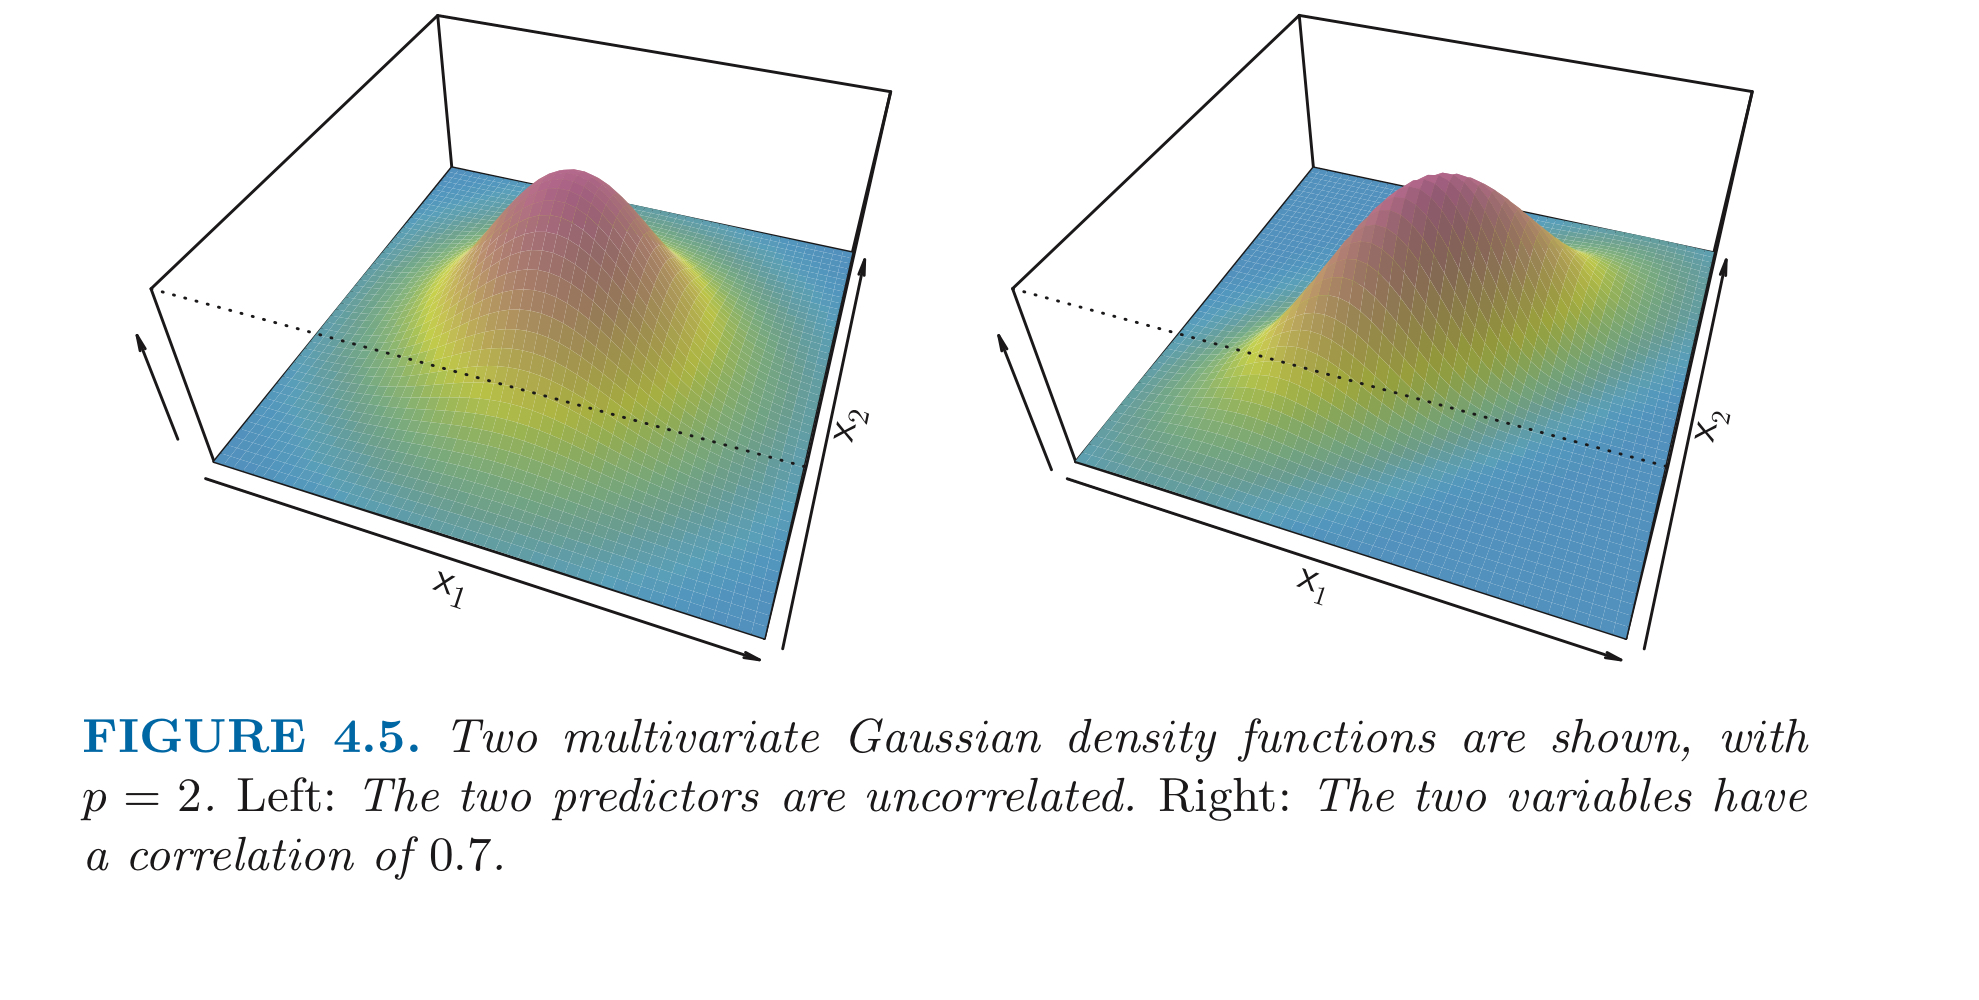
\includegraphics[width=\columnwidth]{MultiVariate Normal.jpeg} % Example image
	\caption{Multivariate Normal Dist}
	\label{multi-normal}
\end{figure}

Think of one dimensional as collapsing into the left side or down. If the var is equal and correlation=0
then the image on the left in \ref{multi-normal} with a circular bottom is produced, if otherwise skewed,
as shown on the right.

\begin{equation}
	X \sim N(\mu,\sum); \mu:\; mean\; vector, \sum:\; covariance\; matrix
\end{equation}

\subsubsection{How is multi preditor LDA used?}

Using the multi variate normal dist values can create the vector/matrix version of the Bayes 
classifier boundary. If there are >2 classes the boundary will be shown as pair of classes.

\subsubsection{Issues to be aware of from multi LDA}

Small distribution between classes in the data set can result in good training error rates, but 
poor test error rates.

\subsection{What is a confusion matrix?}

Determine which type of error is being made in terms of the classes, comparing the error rate for
each class.\\

Sensitivity: Sensitivity is the percentage of true positives (e.g. 90\% sensitivity = 90\% of people who have the target disease will test positive)\\
Specificity: Specificity is the percentage of true negatives (e.g. 90\% specificity = 90\% of people who do not have the target disease will test negative).

\subsection{How to accomdate non equal classes?}

If the bias between classes is not equal the boundary can be altered to instead of being the max,
match the criteria of the problem.

\subsection{What is ROC curve?}

Shows the error rate using different thresholds, the overall peformance of the model is the
area under the curve.\\

If area under the curve is <=0.5 its assumed the performance is no better than chance.

\subsection{Different classification measurments}

\begin{figure}[h] % [h] forces the figure to be output where it is defined in the code (it suppresses floating)
	\centering
	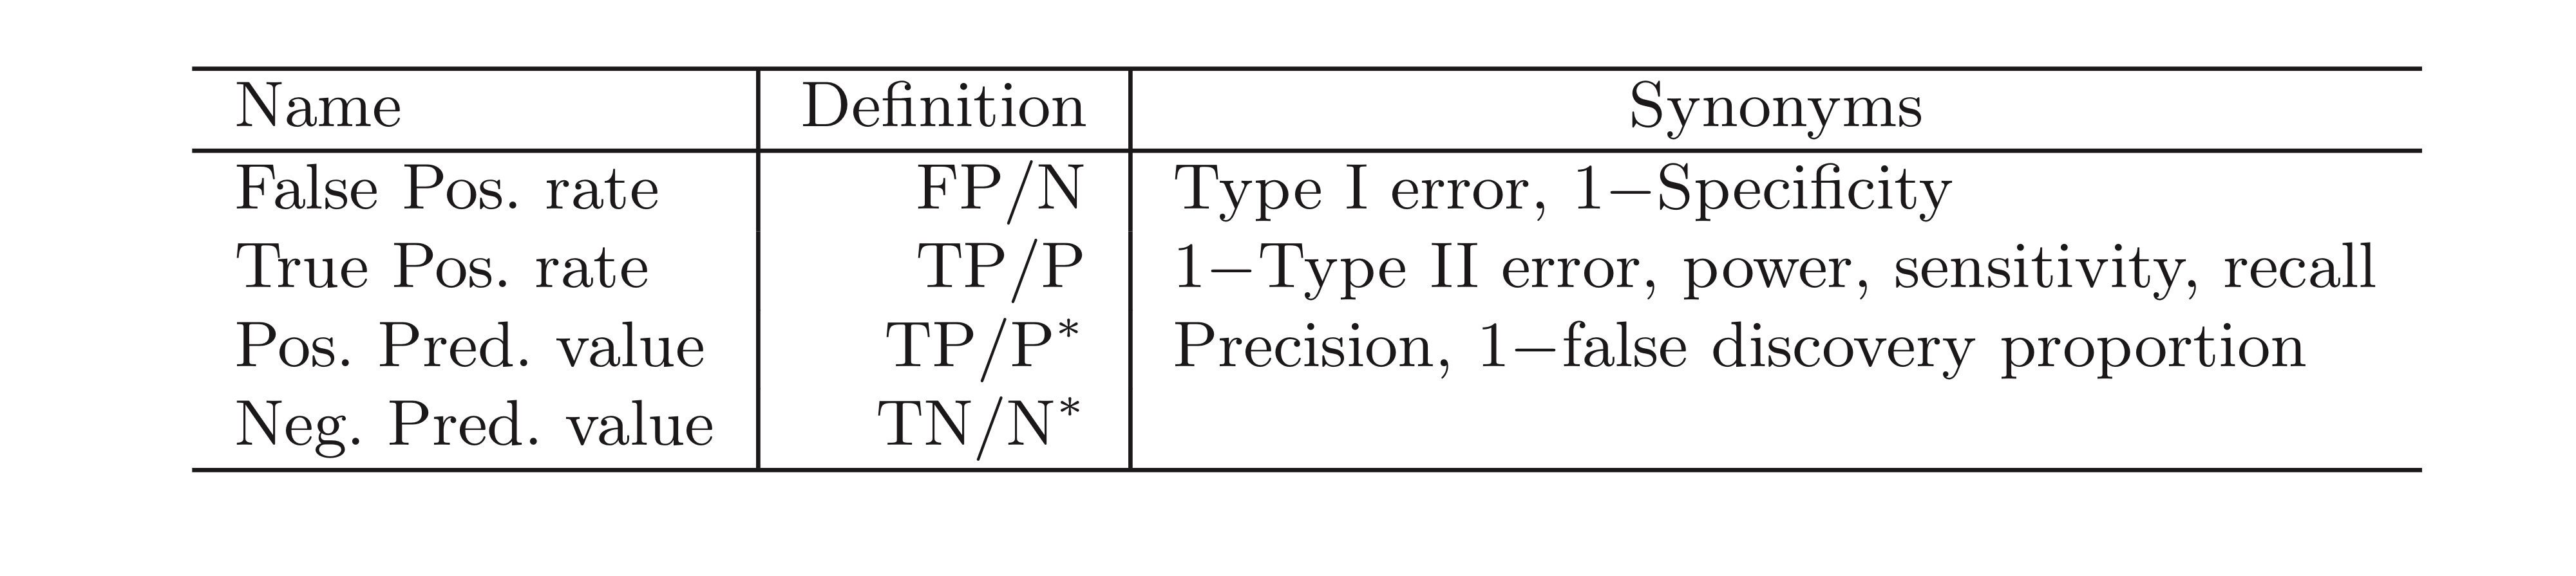
\includegraphics[width=\columnwidth]{classifcation table.jpeg} % Example image
	\caption{Types of classification measurments}
\end{figure}

\subsection{Quadratic Discrimanant Analysis}

The main differnce to LDA is that there is not an assumption of common variance between distribution,
this leads to a quadratic boundary function. 

\subsubsection{What are the pros/cons of QDA?}

More flexiblie, accomdates differing class distributions and therefore has lower bias.\\

It is more compute intensive and has higher variance.

\subsubsection{How do you choose between LDA and QDA?}

Compare the correlation between class and observations for each class, if they are all similar shows
the variance is likley similar. And thefore LDA is a good choice otherwise QDA is.

\subsection{How do you choose between LDA and Logistic for binary scenarios?}

Main differntial is that LDA assumes normal distribution of class, logistic does not.

\subsection{Differences with KNN?}

Descion boundaries cant be weigted towards classes, however it is the most flexible choice.

\subsection{Methods to improve non linear performance?}

Can improve non linear peformance by adding transformed predictors, ie \(X_1^2,X_2^2\) etc.

\section{Resampling methods}

Completley seperate data as the test set may not make sense to use as that could be used as
a valuable method to train the orignial data set. So instead you can repeatadley draw samples
from the data set you have and refit the model and compare to other samples as test data to gain
info about the models setup.\\

\textbf{Model assessment:} Evaluating a models performance.

\textbf{Model selection:} Determining a models flexibilty.\\

\textit{Side note: Can determine if a transformation is valid using hypothesis tests.}

\subsection{Cross Validation}

\subsubsection{What is the validation set approach?}

Randomly divide the data into a training and test set. The issue is there will be less data used
for training the model with each split, will most likley overestimate the test error.

\subsubsection{What is leave one out cross valiation (LOOCV)?}

Use a single observation as the validation set, the rest as training and loop through all data points.

Use the average MSE from all models and validations point:

\begin{equation}
	CV_n = \frac{1}{n} \sum MSE
\end{equation}

The benefits to this are:
\begin{enumerate}
	\item less bias in model as the training set is much bigger
	\item No randomness in method so consistent results produced
\end{enumerate}

This is a very flexible method, however, does require large computation.

\subsubsection{What is K fold cross validation?}

Seperate into K sets, 1 set is the validation and the rest are used for training. Loop through switching
the validation set to each Kth set, taking the average across n sets as the error. 
The main benefit is the computational costs.

Generally the result produced for using K as a reasonable number (>5), produces a result similar to
LOOCV (K=n).\\

The mean of many highly correlated samples has a higher variance than if uncorrelated. And therefore
kCV will produce a low variance than LOOCV but higher bias (less training data used).\\

A good var-bias balance is found around k=5 and k=10, and cleaner to use a multipe of the n as k.
K fold is the main method to compare different models looking for the the bottom of the error over the
different models.

\subsection{Bootstrap}



%----------------------------------------------------------------------------------------
%	FIGURE EXAMPLE
%----------------------------------------------------------------------------------------

% \begin{figure}[h] % [h] forces the figure to be output where it is defined in the code (it suppresses floating)
% 	\centering
% 	\includegraphics[width=0.5\columnwidth]{IMAGE_NAME.jpg} % Example image
% 	\caption{European swallow.}
% \end{figure}

%----------------------------------------------------------------------------------------
% MATH EXAMPLES
%----------------------------------------------------------------------------------------

% \begin{align} 
% 	\label{eq:bayes}
% 	\begin{split}
% 		P(A|B) = \frac{P(B|A)P(A)}{P(B)}
% 	\end{split}					
% \end{align}

%----------------------------------------------------------------------------------------
%	LIST EXAMPLES
%----------------------------------------------------------------------------------------

% \begin{itemize}
% 	\item First item in a list 
% 		\begin{itemize}
% 		\item First item in a list 
% 			\begin{itemize}
% 			\item First item in a list 
% 			\item Second item in a list 
% 			\end{itemize}
% 		\item Second item in a list 
% 		\end{itemize}
% 	\item Second item in a list 
% \end{itemize}

%------------------------------------------------

% \subsection{Numbered List}

% \begin{enumerate}
% 	\item First item in a list 
% 	\item Second item in a list 
% 	\item Third item in a list
% \end{enumerate}

%----------------------------------------------------------------------------------------
%	TABLE EXAMPLE
%----------------------------------------------------------------------------------------

% \section{Interpreting a Table}

% \begin{table}[h] % [h] forces the table to be output where it is defined in the code (it suppresses floating)
% 	\centering % Centre the table
% 	\begin{tabular}{l l l}
% 		\toprule
% 		\textit{Per 50g} & \textbf{Pork} & \textbf{Soy} \\
% 		\midrule
% 		Energy & 760kJ & 538kJ\\
% 		Protein & 7.0g & 9.3g\\
% 		\bottomrule
% 	\end{tabular}
% 	\caption{Sausage nutrition.}
% \end{table}

%----------------------------------------------------------------------------------------
%	CODE LISTING EXAMPLE
%----------------------------------------------------------------------------------------

% \begin{lstlisting}[
% 	caption= Macro definition, % Caption above the listing
% 	language=python, % Use Julia functions/syntax highlighting
% 	frame=single, % Frame around the code listing
% 	showstringspaces=false, % Don't put marks in string spaces
% 	numbers=left, % Line numbers on left
% 	numberstyle=\large, % Line numbers styling
% 	]

% 	CODE

% \end{lstlisting}

%----------------------------------------------------------------------------------------
%	CODE LISTING FILE EXAMPLE
%----------------------------------------------------------------------------------------

% \lstinputlisting[
% 	caption=Luftballons Perl Script., % Caption above the listing
% 	label=lst:luftballons, % Label for referencing this listing
% 	language=Perl, % Use Perl functions/syntax highlighting
% 	frame=single, % Frame around the code listing
% 	showstringspaces=false, % Don't put marks in string spaces
% 	numbers=left, % Line numbers on left
% 	numberstyle=\tiny, % Line numbers styling
% 	]{luftballons.pl}

%------------------------------------------------

\end{document}